%3D Pythagoras - Square based pyramid

\documentclass[tikz,border=10pt]{standalone}
\usepackage{tikz}
\usetikzlibrary{3d} % for 3d vector calculations

\begin{document}

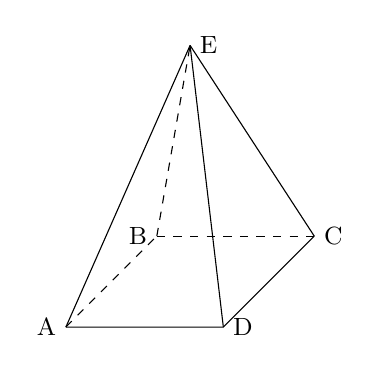
\begin{tikzpicture}[scale=1, transform shape]
    % Define the points of the cube
    \coordinate (A) at (0,0,0);
    \coordinate (B) at (0,0,-3);
    \coordinate (C) at (2,0,-3);
    \coordinate (D) at (2,0,0);
    \coordinate (E) at (1,3,-1.5);

    % Draw the visible edges of the cube
    \draw[dashed] (A) -- (B);
    \draw[dashed] (B) -- (C);
    \draw (A) -- (D) -- (C);
    \draw (A) -- (E);
    \draw[dashed] (B) -- (E);
    \draw (C) -- (E);
    \draw (D) -- (E);

    % Draw the hidden edges of the cube

    % Place the labels with smaller font size
    \node at (A) [left,font=\small] {A};
    \node at (B) [left,font=\small] {B};
    \node at (C) [right,font=\small] {C};
    \node at (D) [right,font=\small] {D};
    \node at (E) [right,font=\small] {E};
\end{tikzpicture}

\end{document}